
\chapter{TangoATK Programmer's Guide}

This chapter is only a brief Tango ATK (Application ToolKit) programmer's
guide. You can find a reference guide with a full description of TangoATK
classes and methods in the ATK JavaDoc \cite{ATK-doc}.

A tutorial document \cite{ATK-Tutorial} is also provided and includes
the detailed description of the ATK architecture and the ATK components.
In the ATK Tutorial \cite{ATK-Tutorial} you can find some code examples
and also Flash Demos which explain how to start using Tango ATK.


\section{Introduction}

This document describes how to develop applications using the Tango
Application Toolkit, TangoATK for short. It will start with a brief
description of the main concepts behind the toolkit, and then continue
with more practical, real-life examples to explain key parts.


\subsection{Assumptions}

The author assumes that the reader has a good knowledge of the Java
programming language, and a thorough understanding of object-oriented
programming. Also, it is expected that the reader is fluent in all
aspects regarding Tango devices, attributes, and commands.


\section{The key concepts of TangoATK}

TangoATK was developed with these goals in mind
\begin{itemize}
\item TangoATK should help minimize development time 
\item TangoATK should help minimize bugs in applications 
\item TangoATK should support applications that contain attributes and commands
from several different devices. 
\item TangoATK should help avoid code duplication. 
\end{itemize}
Since most Tango-applications were foreseen to be displayed on some
sort of graphic terminal, TangoATK needed to provide support for some
sort of graphic building blocks. To enable this, and since the toolkit
was to be written in Java, we looked to Swing to figure out how to
do this.

Swing is developed using a variant over a design-pattern the Model-View-Controller\index{Model-View-Controller}
(MVC\index{MVC}) pattern called \emph{model-delegate}, where the
view and the controller of the MVC-pattern are merged into one object.

\begin{center}
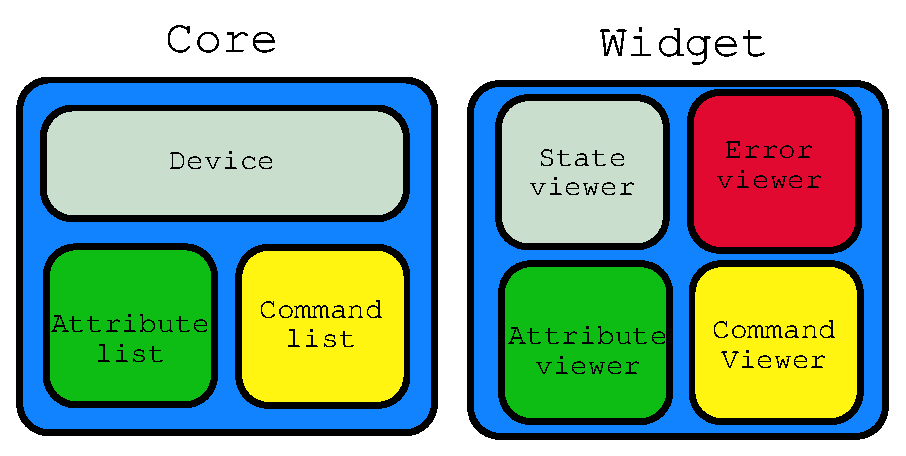
\includegraphics[scale=0.6]{atk/img/core-widget}\\

\par\end{center}

This pattern made the choice of labor division quite easy: all non-graphic
parts of TangoATK reside in the packages beneath \texttt{fr.esrf.tangoatk.core}\index{model}\index{core},
and anything remotely graphic are located beneath \texttt{fr.esrf.tangoatk.widge}t\index{viewer}\index{widget}.
More on the content and organization of this will follow.

The communication between the non-graphic and graphic objects are
done by having the graphic object registering itself as a listener
to the non-graphic object, and the non-graphic object emmiting events
telling the listeners that its state has changed.


\subsection{Minimize development time}

For TangoATK to help minimize the development time of graphic applications,
the toolkit has been developed along two lines of thought
\begin{itemize}
\item Things that are needed in most applications are included, eg \texttt{Splash},
a splash\index{splash} window which gives a graphical way for the
application to show the progress of a long operation. The splash window
is moslty used in the startup phase of the application.
\item Building blocks provided by TangoATK should be easy to use and follow
certain patterns, eg every graphic widget has a \texttt{setModel}
method which is used to connect the widget with its non-graphic model. 
\end{itemize}
In addition to this, TangoATK provides a framework for error handling,
something that is often a time consuming task.


\subsection{Minimize bugs in applications}

Together with the Tango API, TangoATK takes care of most of the hard
things related to programming with Tango. Using TangoATK the developer
can focus on developing her application, not on understanding Tango.


\subsection{Attributes and commands from different devices}

To be able to create applications with attributes\index{attributes}
and commands\index{commands} from different devices, it was decided
that the central objects of TangoATK were not to be the device\index{device},
but rather the \emph{attributes and the commands}. This will certainly
feel a bit awkward at first, but trust me, the design holds.

For this design to be feasible, a structure was needed to keep track
of the commands and attributes, so the \emph{command-list\index{command-list}
and the attribute-list\index{attribte-list}} was introduced. These
two objects can hold commands and attributes from any number of devices.


\subsection{Avoid code duplication}

When writing applications for a control-system without a framework
much code is duplicated. Anything from simple widgets for showing
numeric values to error handling has to be implemented each time.
TangoATK supplies a number of frequently used widgets along with a
framework for connecting these widgets with their non-graphic counterparts.
Because of this, the developer only needs to write the \emph{glue}
- the code which connects these objects in a manner that suits the
specified application.


\section{The real getting started}

Generally there are two kinds of end-user applications: Applications
that only know how to treat one device, and applications that treat
many devices.


\subsection{Single device applications}

Single device applications are quite easy to write, even with a gui.
The following steps are required
\begin{enumerate}
\item Instantiate an AttributeList\index{AttributeList} and fill it with
the attributes you want. 
\item Instantiate a CommandList\index{CommandList} and fill it with the
commands you want. 
\item Connect the whole \emph{AttributeList} with a \emph{list viewer} and
/ or each \emph{individual attribute} with an \emph{attribute viewer}. 
\item Connect the whole \emph{CommandList} to a \emph{command list viewer}
and / or connect each \emph{individual command} in the command list
with a \emph{command viewer}. 
\end{enumerate}
\begin{center}
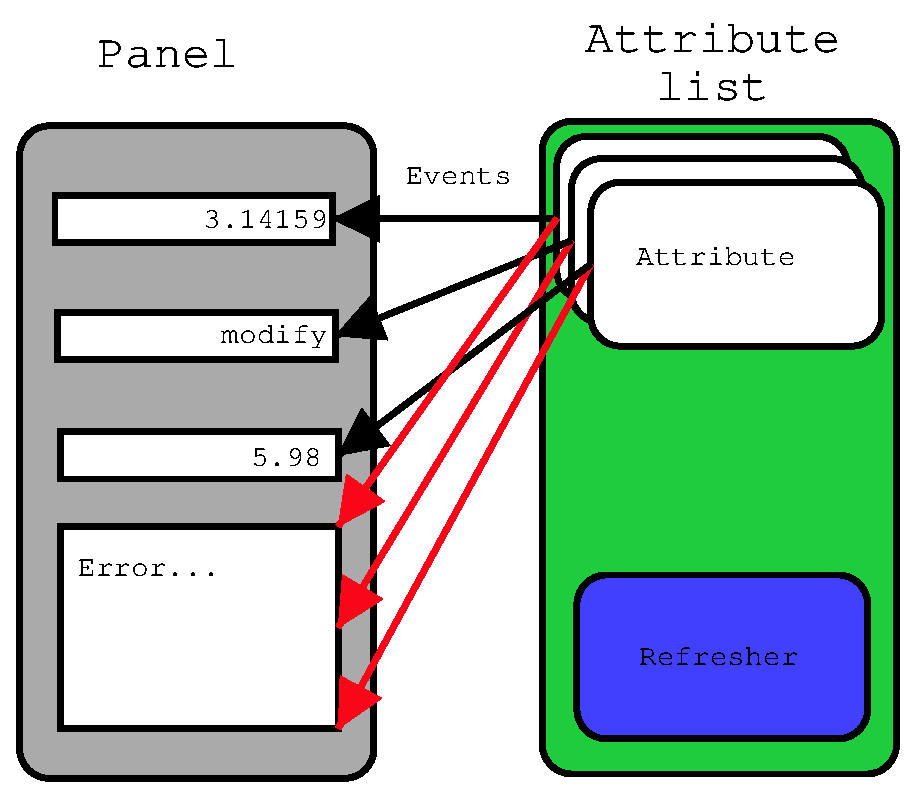
\includegraphics[scale=0.6]{atk/img/listpanel}
\par\end{center}

The following program (FirstApplication)\index{ScalarListViewer}
shows an implementation of the list mentioned above. It should be
rather self-explanatory with the comments.


\begin{minted}[linenos]{cpp}
package examples;
 

import javax.swing.JFrame;
import javax.swing.JMenuItem;
import javax.swing.JMenuBar;
import javax.swing.JMenu;
 

import java.awt.event.ActionListener;
import java.awt.event.ActionEvent;
import java.awt.BorderLayout;
 

import fr.esrf.tangoatk.core.AttributeList;
import fr.esrf.tangoatk.core.ConnectionException;
 

import fr.esrf.tangoatk.core.CommandList;
import fr.esrf.tangoatk.widget.util.ErrorHistory;
import fr.esrf.tangoatk.widget.util.ATKGraphicsUtils;
import fr.esrf.tangoatk.widget.attribute.ScalarListViewer;
import fr.esrf.tangoatk.widget.command.CommandComboViewer;
 

public class FirstApplication extends JFrame
{
JMenuBar menu;                    // So that our application looks
                                  // halfway decent.
AttributeList attributes;         // The list that will contain our
                                  // attributes
CommandList commands;             // The list that will contain our
                                  // commands
ErrorHistory errorHistory;        // A window that displays errors
ScalarListViewer sListViewer;     // A viewer which knows how to
                                  // display a list of scalar attributes.
                                  // If you want to display other types
                                  // than scalars, you'll have to wait
                                  // for the next example.
CommandComboViewer commandViewer; // A viewer which knows how to display
                                  // a combobox of commands and execute
                                  // them.
String device;                    // The name of our device.
 

public FirstApplication()
{
   // The swing stuff to create the menu bar and its pulldown menus
   menu = new JMenuBar();
   JMenu fileMenu = new JMenu();
   fileMenu.setText("File");   
   JMenu viewMenu = new JMenu();
   viewMenu.setText("View");

   JMenuItem quitItem = new JMenuItem();
   quitItem.setText("Quit");
   quitItem.addActionListener(new 
      java.awt.event.ActionListener()
      {                 
       public void
       actionPerformed(ActionEvent evt)
       {quitItemActionPerformed(evt);}
      });
   fileMenu.add(quitItem);

   JMenuItem errorHistItem = new JMenuItem();
   errorHistItem.setText("Error History");
   errorHistItem.addActionListener(new 
           java.awt.event.ActionListener()
           {                 
            public void 
            actionPerformed(ActionEvent evt)
            {errHistItemActionPerformed(evt);}
           });
   viewMenu.add(errorHistItem);
   menu.add(fileMenu);
   menu.add(viewMenu);

   //
   // Here we create ATK objects to handle attributes, commands and errors.
   //
   attributes = new AttributeList(); 
   commands = new CommandList();
   errorHistory = new ErrorHistory();
   device = "id14/eh3_mirror/1";
   sListViewer = new ScalarListViewer();
   commandViewer = new CommandComboViewer();


// 
// A feature of the command and attribute list is that if you
// supply an errorlistener to these lists, they'll add that
// errorlistener to all subsequently created attributes or
// commands. So it is important to do this _before_ you
// start adding attributes or commands.
//
 
   attributes.addErrorListener(errorHistory);
   commands.addErrorListener(errorHistory);
 
//
// Sometimes we're out of luck and the device or the attributes
// are not available. In that case a ConnectionException is thrown.
// This is why we add the attributes in a try/catch
//
 
   try
   {
 
//
// Another feature of the attribute and command list is that they
// can add wildcard names, currently only `*' is supported.
// When using a wildcard, the lists will add all commands or
// attributes available on the device.
//
   attributes.add(device + "/*");
   }
   catch (ConnectionException ce)
   {
      System.out.println("Error fetching " + 
                         "attributes from " +
                         device + " " + ce);
   }
 

//
// See the comments for attributelist
//
 

   try
   {
      commands.add(device + "/*");
   }
   catch (ConnectionException ce)
   {
      System.out.println("Error fetching " +
                         "commands from " +
                         device + " " + ce);
   }
 

//
// Here we tell the scalarViewer what it's to show. The
// ScalarListViewer loops through the attribute-list and picks out
// the ones which are scalars and show them.
//

   sListViewer.setModel(attributes);
 

//
// This is where the CommandComboViewer is told what it's to
// show. It knows how to show and execute most commands.
//
 

   commandViewer.setModel(commands);
 

//
// add the menubar to the frame
//
 

   setJMenuBar(menu);
 

//
// Make the layout nice.
//
 

   getContentPane().setLayout(new BorderLayout());
   getContentPane().add(commandViewer, BorderLayout.NORTH);
   getContentPane().add(sListViewer, BorderLayout.SOUTH);
 

//
// A third feature of the attributelist is that it knows how
// to refresh its attributes.
//
 

   attributes.startRefresher();
 

//
// JFrame stuff to make the thing show.
//
 

   pack();
   ATKGraphicsUtils.centerFrameOnScreen(this); //ATK utility to center window

   setVisible(true);
   }
 

   public static void main(String [] args)
   {
      new FirstApplication();
   }

   public void quitItemActionPerformed(ActionEvent evt)
   {
      System.exit(0);
   }

   public void errHistItemActionPerformed(ActionEvent evt)
   {
      errorHistory.setVisible(true);
   }
}



\end{minted}


The program should look something like this (depending on your platform
and your device)

\begin{center}
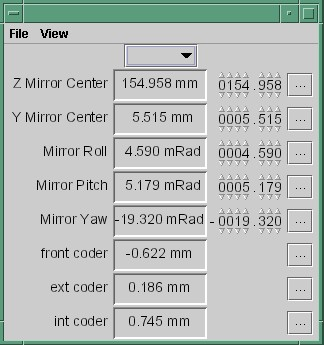
\includegraphics[scale=0.75]{atk/img/prog_guide_exple1}
\par\end{center}


\subsection{Multi device applications}

Multi device applications are quite similar to the single device applications,
the only difference is that it does not suffice to add the attributes
by wildcard, you need to add them explicitly, like this: \\



\begin{minted}[linenos]{cpp}
try
{ 
    // a StringScalar attribute from the device one
   attributes.add("jlp/test/1/att_cinq");
   // a NumberSpectrum attribute from the device one
   attributes.add("jlp/test/1/att_spectrum");
   // a NumberImage attribute from the device two
   attributes.add("sr/d-ipc/id25-1n/Image");
}
catch (ConnectionException ce)
{
   System.out.println("Error fetching " + 
       "attributes" + ce);
}

\end{minted}


The same goes for commands.


\subsection{More on displaying attributes}

So far, we've only considered scalar\index{scalar} attributes, and
not only that, we've also cheated quite a bit since we just passed
the attribute list to the \texttt{fr.esrf.tangoatk.widget.attribute.ScalarListViewer}
and let it do all the magic. The attribute list viewers are only available
for scalar attributes (NumberScalarListViewer\index{NumberScalarListViewer}
and ScalarListViewer\index{ScalarListViewer}). If you have one or
several spectrum\index{spectrum} or image\index{image} attributes
you must connect each spectrum or image attribute to it's corresponding
attribute viewer individually. So let's take a look at how you can
connect individual attributes (and not a whole attribute list) to
an individual attribute viewer (and not to an attribute list viewer).


\subsubsection{Connecting an attribute\index{model} to a viewer\index{viewer}}

Generally it is done in the following way:
\begin{enumerate}
\item You retrieve the attribute from the attribute list 
\item You instantiate the viewer 
\item Your call the \texttt{setModel\index{setModel}} method on the viewer
with the attribute as argument. 
\item You add your viewer to some panel
\end{enumerate}
The following example (SecondApplication)\index{SimpleScalarViewer}\index{NumberImageViewer}\index{NumberSpectrumViewer},
is a Multi-device application. Since this application uses individual
attribute viewers and not an attribute list viewer, it shows an implementation
of the list mentioned above.


\begin{minted}[linenos]{cpp}
package examples;
 

import javax.swing.JFrame;
import javax.swing.JMenuItem;
import javax.swing.JMenuBar;
import javax.swing.JMenu;
 

import java.awt.event.ActionListener;
import java.awt.event.ActionEvent;
import java.awt.BorderLayout;
import java.awt.Color;
 

import fr.esrf.tangoatk.core.AttributeList;
import fr.esrf.tangoatk.core.ConnectionException;
 
import fr.esrf.tangoatk.core.IStringScalar;
import fr.esrf.tangoatk.core.INumberSpectrum;
import fr.esrf.tangoatk.core.INumberImage;
import fr.esrf.tangoatk.widget.util.ErrorHistory;
import fr.esrf.tangoatk.widget.util.Gradient;
import fr.esrf.tangoatk.widget.util.ATKGraphicsUtils;
import fr.esrf.tangoatk.widget.attribute.NumberImageViewer;
import fr.esrf.tangoatk.widget.attribute.NumberSpectrumViewer;
import fr.esrf.tangoatk.widget.attribute.SimpleScalarViewer;

public class SecondApplication extends JFrame
{
     JMenuBar            menu;
     AttributeList       attributes;   // The list that will contain our attributes
     ErrorHistory        errorHistory; // A window that displays errors
     IStringScalar        ssAtt;
     INumberSpectrum      nsAtt;
     INumberImage         niAtt;
     public SecondApplication()
     {
        // Swing stuff to create the menu bar and its pulldown menus
        menu = new JMenuBar();
        JMenu fileMenu = new JMenu();
        fileMenu.setText("File");   
        JMenu viewMenu = new JMenu();
        viewMenu.setText("View");
        JMenuItem quitItem = new JMenuItem();
        quitItem.setText("Quit");
        quitItem.addActionListener(new java.awt.event.ActionListener()
                                      {                 
                                       public void actionPerformed(ActionEvent evt)
                                       {quitItemActionPerformed(evt);}
                                      });

        fileMenu.add(quitItem);
        JMenuItem errorHistItem = new JMenuItem();
        errorHistItem.setText("Error History");
        errorHistItem.addActionListener(new java.awt.event.ActionListener()
                {                 
                 public void actionPerformed(ActionEvent evt)
                 {errHistItemActionPerformed(evt);}
                });
        viewMenu.add(errorHistItem);
        menu.add(fileMenu);
        menu.add(viewMenu);
      //
      // Here we create TangoATK objects to view attributes and errors.
      //
        attributes = new AttributeList(); 
        errorHistory = new ErrorHistory();
      //
      // We create a SimpleScalarViewer, a NumberSpectrumViewer and
      // a NumberImageViewer, since we already knew that we were
      // playing with a scalar attribute, a number spectrum attribute
      // and a number image attribute this time.
      //
      SimpleScalarViewer     ssViewer = new SimpleScalarViewer();
        NumberSpectrumViewer   nSpectViewer = new NumberSpectrumViewer();
        NumberImageViewer      nImageViewer = new NumberImageViewer();
        attributes.addErrorListener(errorHistory);
     //
     // The attribute (and command) list has the feature of returning the last
     // attribute that was added to it. Just remember that it is returned as an
     // IEntity object, so you need to cast it into a more specific object, like
     // IStringScalar, which is the interface which defines a string scalar
     //
       try
        {

           ssAtt = (IStringScalar) attributes.add("jlp/test/1/att_cinq");
           nsAtt = (INumberSpectrum) attributes.add("jlp/test/1/att_spectrum");
           niAtt = (INumberImage) attributes.add("sr/d-ipc/id25-1n/Image");
        }
        catch (ConnectionException ce)
        {
           System.out.println("Error fetching one of the attributes  "+" " + ce);
           System.out.println("Application Aborted.");
           System.exit(0);
        }        
        //
        // Pay close attention to the following three lines!! This is how it's done!
        // This is how it's always done! The setModelsetModel method of any viewer takes care
       // of connecting the viewer to the attribute (model) it's in charge of displaying.
       // This is the way to tell each viewer what (which attribute) it has to show.
       // Note that we use a viewer adapted to each type of attribute
       //
        ssViewer.setModel(ssAtt);
        nSpectViewer.setModel(nsAtt);
        nImageViewer.setModel(niAtt);
     //
        nSpectViewer.setPreferredSize(new java.awt.Dimension(400, 300));
        nImageViewer.setPreferredSize(new java.awt.Dimension(500, 300));
        Gradient  g = new Gradient();
        g.buidColorGradient();
        g.setColorAt(0,Color.black);
        nImageViewer.setGradient(g);
        nImageViewer.setBestFit(true);

        //
        // Add the viewers into the frame to show them
        //
        getContentPane().setLayout(new BorderLayout());
        getContentPane().add(ssViewer, BorderLayout.SOUTH);
        getContentPane().add(nSpectViewer, BorderLayout.CENTER);
        getContentPane().add(nImageViewer, BorderLayout.EAST);
        //
        // To have the attributes values refreshed we should start the
        // attribute list's refresher.
        //
        attributes.startRefresher();
        //
        // add the menubar to the frame
        //
        setJMenuBar(menu);
        //
        // JFrame stuff to make the thing show.
        //
        pack();
        ATKGraphicsUtils.centerFrameOnScreen(this); //ATK utility to center window
        setVisible(true);
     }
     public static void main(String [] args)
     {
        new SecondApplication();
     }
     public void quitItemActionPerformed(ActionEvent evt)
     {
        System.exit(0);
     }
     public void errHistItemActionPerformed(ActionEvent evt)
     {
        errorHistory.setVisible(true);
     }
}




\end{minted}


This program (SeondApplication) should look something like this (depending
on your platform and your device attributes)\\


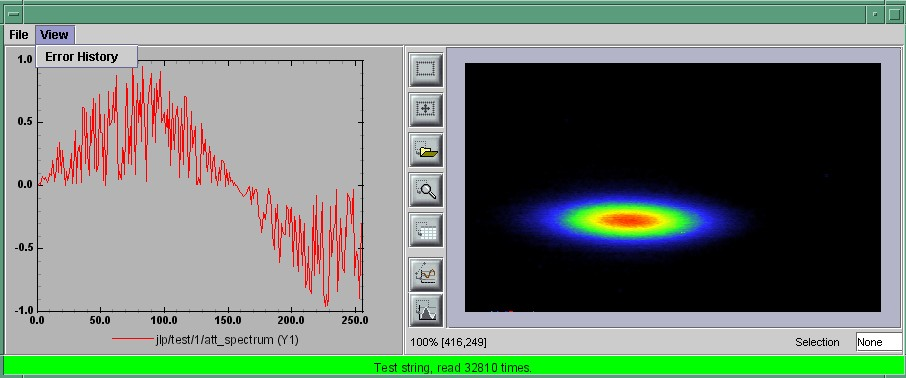
\includegraphics[scale=0.5]{atk/img/prog_guide_exple2}
\begin{minted}[linenos]{cpp}

\end{minted}

\subsubsection{Synoptic\index{Synoptic} viewer}

TangoATK provides a generic class to view and to animate the synoptics.
The name of this class is fr.esrf.tangoatk.widget.jdraw.SynopticFileViewer\index{SynopticFileViewer}.
This class is based on a ``home-made'' graphical layer called jdraw\index{jdraw}.
The jdraw package is also included inside TangoATK distribution.

SynopticFileViewer is a sub-class of the class TangoSynopticHandler.
All the work for connection to tango devices and run time animation
is done inside the TangoSynopticHandler.

The recipe for using the TangoATK synoptic viewer is the following
\begin{enumerate}
\item You use Jdraw graphical editor to draw your synoptic 
\item During drawing phase don't forget to associate parts of the drawing
to tango attributes or commands. Use the ``name'' in the property
window to do this
\item During drawing phase you can also aasociate a class (frequently a
``specific panel'' class) which will be displayed when the user
clicks on some part of the drawing. Use the ``extension'' tab in
the property window to do this.
\item Test the run-time behaviour of your synoptic. Use ``Tango Synoptic
view'' command in the ``views'' pulldown menu to do this.
\item Save the drawing file.
\item There is a simple synoptic application (SynopticAppli) which is provided
ready to use. If this generic application is enough for you, you can
forget about the step 7.
\item You can now develop a specific TangoATK based application which instantiates
the SynopticFileViewer. To load the synoptic file in the SynopticFileViewer
you have the choice : either you load it by giving the absolute path
name of the synoptic file or you load the synoptic file using Java
input streams. The second solution is used when the synoptic file
is included inside the application jarfile.
\end{enumerate}
The SynopticFilerViewer will browse the objects in the synoptic file
at run time. It discovers if some parts of the drawing is associated
with an attribute or a command. In this case it will automatically
connect to the corresponding attribute or command. Once the connection
is successfull SynopticFileViewer will animate the synoptic according
to the default behaviour described below :
\begin{itemize}
\item For \emph{tango state attributes} : the colour of the drawing object
reflects the value of the state. A mouse click on the drawing object
associated with the tango state attribute will instantiate and display
the class specified during the drawing phase. If no class is specified
the atkpanel generic device panel is displayed.
\item For \emph{tango attributes\index{attributes}} : the current value
of the attribute is displayed through the drawing object
\item For \emph{tango commands\index{commands}} : the mouse click on the
drawing object associated with the command will launch the device
command.
\item If the tooltip\index{tooltip} property is set to ``name'' when
the mouse enters \emph{any tango object} ( attribute or command),
inside the synoptic drawing the name of the tango object is displayed
in a tooltip.
\end{itemize}
The following example (ThirdApplication), is a Synoptic\index{SynopticFileViewer}\index{Synoptic}
application. We assume that the synoptic has already been drawn using
Jdraw graphical editor.


\begin{minted}[linenos]{cpp}
package examples;
import java.io.*;
import java.util.*;
import javax.swing.JFrame;
import javax.swing.JMenuItem;
import javax.swing.JMenuBar;
import javax.swing.JMenu;
import java.awt.event.ActionListener;
import java.awt.event.ActionEvent;
import java.awt.BorderLayout;
import fr.esrf.tangoatk.widget.util.ErrorHistory;
import fr.esrf.tangoatk.widget.util.ATKGraphicsUtils;
import fr.esrf.tangoatk.widget.jdraw.SynopticFileViewer;
import fr.esrf.tangoatk.widget.jdraw.TangoSynopticHandler;
public class ThirdApplication extends JFrame
{
     JMenuBar              menu;
     ErrorHistory          errorHistory;  // A window that displays errors
     SynopticFileViewer    sfv;           // TangoATK generic synoptic viewer
     
     
     public ThirdApplication()
     {
        // Swing stuff to create the menu bar and its pulldown menus
        menu = new JMenuBar();
        JMenu fileMenu = new JMenu();
        fileMenu.setText("File");   
        JMenu viewMenu = new JMenu();
        viewMenu.setText("View");
        JMenuItem quitItem = new JMenuItem();
        quitItem.setText("Quit");
        quitItem.addActionListener(new java.awt.event.ActionListener()
                                      {                 
                                       public void actionPerformed(ActionEvent evt)
                                       {quitItemActionPerformed(evt);}
                                      });
        fileMenu.add(quitItem);
        JMenuItem errorHistItem = new JMenuItem();
        errorHistItem.setText("Error History");
        errorHistItem.addActionListener(new java.awt.event.ActionListener()
                {                 
                 public void actionPerformed(ActionEvent evt)
                 {errHistItemActionPerformed(evt);}
                });
        viewMenu.add(errorHistItem);
        menu.add(fileMenu);
        menu.add(viewMenu);
        //
        // Here we create TangoATK synoptic viewer and error window.
        //
        errorHistory = new ErrorHistory();
        sfv = new SynopticFileViewer();
        try
        {
            sfv.setErrorWindow(errorHistory);
        }
        catch (Exception setErrwExcept)
        {
            System.out.println("Cannot set Error History Window");
        }

        //      
        // Here we define the name of the synoptic file to show and the tooltip mode to use
        //        
        try
        {     
          sfv.setJdrawFileName("/users/poncet/ATK_OLD/jdraw_files/id14.jdw");
          sfv.setToolTipMode (TangoSynopticHandler.TOOL_TIP_NAME);
        }
        catch (FileNotFoundException  fnfEx)
        {
           javax.swing.JOptionPane.showMessageDialog(
              null, "Cannot find the synoptic file : id14.jdw.\n"
                   + "Check the file name you entered;"
                   + " Application will abort ...\n"
                   + fnfEx,
                   "No such file",
                   javax.swing.JOptionPane.ERROR_MESSAGE);
           System.exit(-1);
        }
        catch (IllegalArgumentException  illEx)
        {
           javax.swing.JOptionPane.showMessageDialog(
              null, "Cannot parse the synoptic file : id14.jdw.\n"
                   + "Check if the file is a Jdraw file."
                   + " Application will abort ...\n"
                   + illEx,
                   "Cannot parse the file",
                   javax.swing.JOptionPane.ERROR_MESSAGE);
           System.exit(-1);
        }
        catch (MissingResourceException  mrEx)
        {
           javax.swing.JOptionPane.showMessageDialog(
              null, "Cannot parse the synoptic file : id14.jdw.\n"
                   + " Application will abort ...\n"
                   + mrEx,
                   "Cannot parse the file",
                   javax.swing.JOptionPane.ERROR_MESSAGE);
           System.exit(-1);
        }
        //
        // Add the viewers into the frame to show them
        //
        getContentPane().setLayout(new BorderLayout());
        getContentPane().add(sfv, BorderLayout.CENTER);
        //
        // add the menubar to the frame
        //
        setJMenuBar(menu);
        //
        // JFrame stuff to make the thing show.
        //
        pack();
        ATKGraphicsUtils.centerFrameOnScreen(this); //TangoATK utility to center window
        setVisible(true);
     }
     public static void main(String [] args)
     {
        new ThirdApplication();
     }
     public void quitItemActionPerformed(ActionEvent evt)
     {
        System.exit(0);
     }
     public void errHistItemActionPerformed(ActionEvent evt)
     {
        errorHistory.setVisible(true);
     }
}
[Input: line.tex]


\end{minted}
The synoptic\index{synoptic} application (ThirdApplication) should
look something like this (depending on your synoptic drawing file)\\
\\
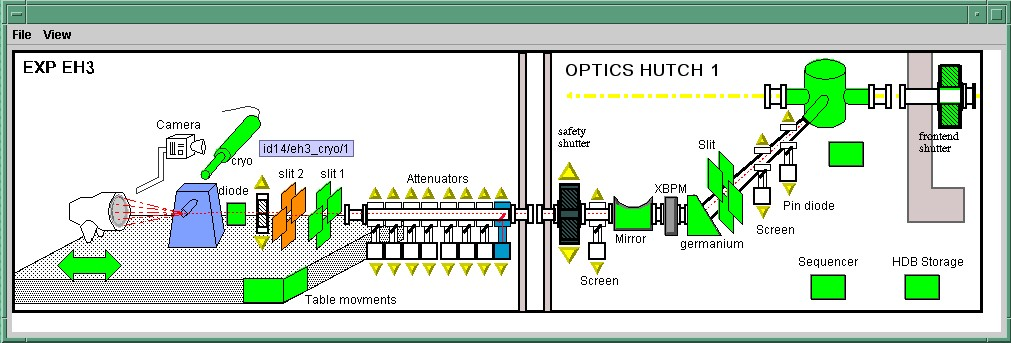
\includegraphics[scale=0.4]{atk/img/prog_guide_exple3}


\subsection{A short note on the relationship between models and viewers}

As seen in the examples above, the connection between a model\index{model}
and its viewer\index{viewer} is generally done by calling \texttt{setModel\index{setModel}(model\index{model})}
on the viewer\index{viewer}, it is never explained what happens behind
the scenes when this is done.


\subsubsection{Listeners}

Most of the viewers\index{viewer} implement some sort of \emph{listener\index{listener}}
interface, eg INumberScalarListener\index{INumberScalarListener}.
An object implementing such a listener interface has the capability
of receiving and treating \emph{events\index{event}} from a model\index{model}
which emits events.


\begin{minted}[linenos]{cpp}
// this is the setModel of a SimpleScalarViewer
  public void setModelsetModel(INumberScalar scalar) {

    clearModel();

    if (scalar != null) {
      format = scalar.getProperty("format").getPresentation();
      numberModel = scalar;
 
   // this is where the viewer connects itself to the 
   // model. After this the viewer will (hopefully) receive 
   // events through its numberScalarChange() method

   numberModel.addNumberScalarListener(this);
 
      
        numberModel.getProperty("format").addPresentationListener(this);
      numberModel.getProperty("unit").addPresentationListener(this);
    }

  }
 
 

// Each time the model of this viewer (the numberscalar attribute) decides it is time, it 
// calls the numberScalarChange method of all its registered listeners
// with a NumberScalarEvent object which contains the 
// the new value of the numberscalar attribute.
//
 
  public void numberScalarChange(NumberScalarEvent evt) {
    String val;
    val = getDisplayString(evt);
    if (unitVisible) {
      setText(val + " " + numberModel.getUnit());
    } else {
      setText(val);
    }
  }



\end{minted}


All listeners in TangoATK implement the \texttt{IErrorListener} interface
which specifies the \texttt{errorChange(ErrorEvent e)} method. This
means that all listeners are forced to handle errors in some way or
another.


\section{The key objects of TangoATK}

As seen from the examples above, the key objects of TangoATK are the
\texttt{CommandList\index{CommandList}} and the \texttt{AttributeList}\index{AttributeList}.
These two classes inherit from the abstract class \texttt{AEntityList}
which implements all of the common functionality between the two lists.
These lists use the functionality of the \texttt{CommandFactory},
the \texttt{AttributeFactory}, which both derive from \texttt{AEntityFactory,}
and the \texttt{DeviceFactory}.

In addition to these factories and lists there is one (for the time
being) other important functionality lurking around, the refreshers.


\subsection{The Refreshers}

The refreshers\index{refresher}, represented in TangoATK by the \texttt{Refresher}
object, is simply a subclass of \texttt{java.lang.Thread} which will
sleep for a given amount of time and then call a method refresh on
whatever kind of \texttt{IRefreshee} it has been given as parameter,
as shown below


\begin{minted}[linenos]{cpp}
// This is an example from DeviceFactory.
// We create a new Refresher with the name "device"
// We add ourself to it, and start the thread
 

Refresher refresher = new Refresher("device");
refresher.addRefreshee(this).start();

\end{minted}


Both the \texttt{AttributeList\index{AttributeList}} and the \texttt{DeviceFactory}
implement the \texttt{IRefreshee} interface which specify only one
method, \texttt{refresh()}, and can thus be refreshed by the \texttt{Refresher}\index{refresher}.
Even if the new release of TangoATK is based on the Tango Events\index{event}\index{Tango-Event},
the refresher mecanisme will not be removed. As a matter of fact,
the method refresh() implemented in \noun{AttributeList} skips all
attributes (members of the list) for which the subscribe\index{subscribe}
to the tango event has succeeded and calls the old refresh() method
for the others (for which subscribe to tango events has failed). 

In a first stage this will allow the TangoATK applications to mix
the use of the old tango device servers (which do not implement tango
events) and the new ones in the same code. In other words, TangoATK
subscribes for tango events if possible otherwise TangoATK will refresh
the attributes through the old refresher mecanisme.

Another reason for keeping the refresher is that the subscribe event
can fail even for the attributes of the new Tango device servers.
As soon as the specified attribute is not polled the Tango events
cannot be generated for that attribute. Therefore the event subscription
will fail. In this case the attribute will be refreshed thanks to
the ATK attribute list refresher.

The \texttt{AttributePolledList} class allows the application programmer
to force explicitly the use of the refresher method for all attributes
added in an AttributePolledList even if the corresponding device servers
implement tango events. Some viewers (fr.esrf.tangoatk.widget.attribute.Trend)
need an AttributePolledList in order to force the refresh of the attribute
without using tango events.


\subsubsection{What happens on a refresh}

When \texttt{refresh\index{refresh}} is called on the \texttt{AttributeList}
and the \texttt{DeviceFactory}, they loop through their objects, \texttt{IAttributes}
and \texttt{IDevices}, respectively, and ask them to refresh themselves
if they are not event driven.

When \noun{AttributeFactory}, creates an \texttt{IAttribute}, TangoATK
tries to subscribe for Tango Change event for that attribute. If the
subscription succeeds then the attribute is marked as event driven.
If the subscription for Tango Change event fails, TangoATK tries to
subscribe for Tango Periodic event. If the subscription succeeds then
the attribute is marked as event driven. If the subscription fails
then the attribute is marked as to be `` without events''.

In the \noun{refresh()} method of the \noun{AttributeList} during
the loop through the objects if the object is marked event driven
then the object is simply skipped. But if the object (attribute) is
not marked as event driven, the \noun{refresh()} method of the \noun{AttributeList},
asks the object to refresh itself by calling the ``\noun{refresh()}''
method of that object (attribute or device). The \noun{refresh()}
method of an attribute will in turn call the ``readAttribute'' on
the Tango device.

The result of this is that the \texttt{IAttributes} fire off events
to their registered listeners\index{listener} containing snapshots
of their state. The events are fired either because the \noun{IAttribute}
has received a Tango Change event, respectively a Tango Periodic event
(event driven objects), or because the \noun{refresh()} method of
the object has issued a readAttribute on the Tango device.


\subsection{The DeviceFactory}

The device factory is responsible for two things
\begin{enumerate}
\item Creating new devices (Tango device proxies) when needed 
\item Refreshing the state and status of these devices 
\end{enumerate}
Regarding the first point, new devices are created when they are asked
for and only if they have not already been created. If a programmer
asks for the same device twice, she is returned a reference to the
same device-object.

The \texttt{DeviceFactory} contains a Refresher as described above,
which makes sure that the all \textsf{Devices} in the \textsf{DeviceFactory}
updates their state and status and fire events to its listeners.


\subsection{The AttributeFactory and the CommandFactory}

These factories are responsible for taking a name of an attribute
or command and returning an object representing the attribute or command.
It is also responsible for making sure that the appropriate \texttt{IDevice}
is already available. Normally the programmer does not want to use
these factory classes directly. They are used by TangoATK classes
indirectly when the application programmer calls the AttributeList's
(or CommandList's) \noun{add()} method.


\subsection{The AttributeList\index{AttributeList} and the CommandList\index{CommandList}}

These lists are containers for attributes and commands. They delegate
the construction-work to the factories mentioned above, and generally
do not do much more, apart from containing refreshers, and thus being
able to make the objects they contain refresh their listeners.


\subsection{The Attributes}

The attributes\index{attributes} come in several flavors. Tango supports
the following types:
\begin{itemize}
\item Short 
\item Long 
\item Double
\item String 
\item Unsigned Char
\item Boolean
\item Unsigned Short
\item Float
\item Unsigned Long
\end{itemize}
According to Tango specifications, all these types can be of the following
formats:
\begin{itemize}
\item Scalar, a single value 
\item Spectrum, a single array 
\item Image, a two dimensional array 
\end{itemize}
For the sake of simplicity, TangoATK has combined all the numeric
types into one, presenting all of them as doubles. So the TangoATK
classes which handle the numeric attributes are : NumberScalar, NumberSpectrum
and NumberImage (Number can be short, long, double, float, ...).


\subsubsection{The hierarchy}

The numeric attribute hierarchy is expressed in the following interfaces:
\begin{description}
\item [{INumberScalar}] extends \textbf{INumber}
\item [{INumberSpectrum}] extends \textbf{INumber}
\item [{INumberImage}] extends \textbf{INumber}
\item [{\textmd{and}}] \textbf{INumber} in turn extends \textbf{IAttribute}
~
\end{description}
Each of these types emit their proper events and have their proper
listeners. Please consult the javadoc for further information.


\subsection{The Commands}

The commands\index{commands} in Tango are rather ugly beasts. There
exists the following kinds of commands
\begin{itemize}
\item Those which take input 
\item Those which do not take input 
\item Those which do output 
\item Those which do not do output 
\end{itemize}
Now, for both input and output we have the following types:
\begin{itemize}
\item Double 
\item Float
\item Unsigned Long
\item Long 
\item Unsigned Short
\item Short 
\item String
\end{itemize}
These types can appear in scalar or array formats. In addition to
this, there are also four other types of parameters:
\begin{enumerate}
\item Boolean
\item Unsigned Char Array
\item The StringLongArray 
\item The StringDoubleArray 
\end{enumerate}
The last two types mentioned above are two-dimensional arrays containing
a string array in the first dimension and a long or double array in
the second dimension, respectively.

As for the attributes, all numeric types have been converted into
doubles, but there has been made little or no effort to create an
hierarchy of types for the commands.


\subsubsection{Events\index{event} and listeners\index{listener}}

The commands publish results to their \texttt{IResultListener}s, by
the means of a \texttt{ResultEvent}. The \texttt{IResultListener}
extends \texttt{IErrorListener}, any viewer\index{viewer} of command-results
should also know how to handle errors. So a viewer of command-results
implements IResultListener interface and registers itself as a resultListener
for the command it has to show the results.
\begin{minted}[linenos]{cpp}
 


\end{minted}
\begin{center}
\label{TwoRicardo}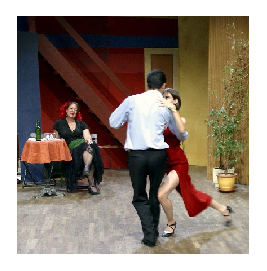
\includegraphics[scale=4]{dance/0046-reduc}
\par\end{center}
